\section{The WSN construction}
\begin{frame}{The WSN construction}
    \centering
    Published by \textcite{AC:Tessaro15} at AsiaCrypt 2015.
    \begin{columns}
        \begin{column}{0.49\textwidth}
            \begin{block}{Overview\vpPp}
                \centering
                \vspace*{13pt}
                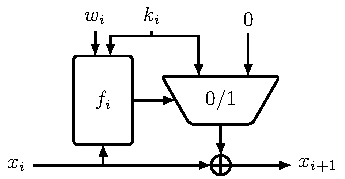
\includegraphics{data/wsn}
                \vspace*{13pt}
            \end{block}
        \end{column}
        \begin{column}{0.49\textwidth}
            \begin{block}{Whitened Swap-Or-Not round function}
                \vspace*{-10pt}
                \begin{equation*}
                    x_i \mapsto x_i + f_{b(i)}(w_i + \max \set{x_i, x_i + k_i}) \cdot k_i
                \end{equation*}
            \end{block}

            \begin{block}{Security Proposition (informal)}
                The WSN construction with $\mathcal{O}(n)$ rounds is
                \begin{equation*}
                    (2^{n-\mathcal{O}(\log n)}, 2^{n-\mathcal{O}(1)})\text{-secure}.
                \end{equation*}
            \end{block}
        \end{column}
    \end{columns}
    \begingroup
        \vspace{10pt}
        \footnotesize
        $(p, q)$-secure: Attackers querying the encryption at most $p$ and the underlying $f_i$'s $q$ times have only negl.\ advantage.
    \endgroup
    \blfootnote{}
\end{frame}

\section{Generic Analysis}
\begin{frame}{Generic Analysis}{On the number of rounds}
    \begin{columns}
        \begin{column}{0.49\textwidth}
            \begin{block}{Observation}
                \begin{itemize}
                    \item The ciphertext is the plaintext plus a random subset of the round keys:
                        \begin{equation*}
                            c = p + \sum_{i=1}^{r} \lambda_i k_i
                        \end{equation*}
                    \item For pairs $p_i, c_i$: $\Span \set{p_i + c_i} \subseteq \Span \set{k_j}$.
                \end{itemize}
            \end{block}
        \end{column}
        \begin{column}{0.49\textwidth}
            \begin{alertblock}{Problematic because}
                \vspace{1.5pt}
                \begin{itemize}
                    \item $\Span \set{k_j} \subset \F_2^n$ reveals information on the round keys\\[7pt]
                    \item for $r < n$ there exists probability one linear hulls (exploitable: easy),\\[7pt]
                    \item for $r < 2n - 3$ there exists zero correlation linear hulls (exploitable: ???).
                \end{itemize}
                \vspace{1.5pt}
            \end{alertblock}
        \end{column}
    \end{columns}
    \hspace*{-8.5pt}
    \begin{minipage}{1.0145\textwidth}
    \begin{exampleblock}{Rationale 1}
        Any instance must iterate at least n rounds; any set of n consecutive keys should be linear indp.
    \end{exampleblock}
    \end{minipage}
\end{frame}

\begin{frame}{Generic Analysis}{On the Boolean functions $f_i$}
    \begin{columns}
        \begin{column}{0.49\textwidth}
            \begin{block}{Observation\vpPp}
                \begin{itemize}
                    \item If the $f_i$ do not depend on a (linear combination of) bit(s), \ie/
                        \begin{equation*}
                            f_i(x) = f_i(x + \delta)
                        \end{equation*}
                        this difference propagates through the whole encryption with non-negligible probability.
                \end{itemize}
            \end{block}
        \end{column}
        \begin{column}{0.49\textwidth}
            \begin{block}{Why could this happen?}
                \begin{itemize}
                    \item For example, when the difference does not influence the lexicographic ordering of $x$ and $x + k_i$.
                \end{itemize}
                \vspace{56pt}
            \end{block}
        \end{column}
    \end{columns}
    \hspace*{-8.5pt}
    \begin{minipage}{1.0145\textwidth}
    \begin{exampleblock}{Rationale 2}
        For any instance, the $f_i$ should depend on all bits, and for any $\delta \in \F_2^n:\ \Pr\bracket{f_i(x) = f_i(x + \delta)} \approx \frac{1}{2}$.
    \end{exampleblock}
    \end{minipage}
\end{frame}

\begin{frame}{Addressing Rationale 1}{The Key Schedule}
    \hspace*{-8.5pt}
    \begin{minipage}{1.0145\textwidth}
    \begin{exampleblock}{Rationale 1}
        Any instance must iterate at least n rounds; any set of n consecutive keys should be linear indp.
    \end{exampleblock}
    \end{minipage}
    \begin{columns}
        \begin{column}{0.49\textwidth}
            \begin{block}{Design Decisions}
                \begin{itemize}
                    \item Choose number of rounds as $2 \cdot n$\\[5pt]
                    \item Round Keys derived from the state of LFSRs\\[5pt]
                    \item Add round constants $c_i$ to $w_i$ round keys
                \end{itemize}
                \vspace{30pt}
            \end{block}
        \end{column}
        \begin{column}{0.49\textwidth}
            \begin{block}{Implications}
                \begin{itemize}
                    \item Clocking an LFSR is cheap
                    \item For an LFSR with feedback polynomial of degree $n$, every $n$ consecutive states are linearly independent
                    \item Round constants avoid structural weaknesses
                \end{itemize}
            \end{block}
        \end{column}
    \end{columns}
\end{frame}

\begin{frame}{Addressing Rationale 2}{The Round Function}
    \hspace*{-8.5pt}
    \begin{minipage}{1.0145\textwidth}
    \begin{exampleblock}{Rationale 2}
        For any instance, the $f_i$ should depend on all bits, and for any $\delta \in \F_2^n:\ \Pr\bracket{f_i(x) = f_i(x + \delta)} \approx \frac{1}{2}$.
    \end{exampleblock}
    \end{minipage}
    \begin{columns}
        \begin{column}{0.49\textwidth}
            \begin{block}{Design Decision}
                \begin{itemize}
                    \item Choose $f_i : \F_2^n \to \F_2$ to be bent
                    \item Replace $x \mapsto \max \set{x, x+k}$ by
                          \begin{align*}
                              \Phi_k(x) : \F_2^n &\to \F_2^{n-1} \\
                              \Phi_k(x) &\coloneqq (x + x[i(k)] \cdot k)[j]_{\tower{1 \leqslant j \leqslant n}{j \neq i(k)}}
                          \end{align*}
                \end{itemize}
            \end{block}
        \end{column}
        \begin{column}{0.49\textwidth}
            \begin{block}{Implications}
                \begin{itemize}
                    \item With $\Phi_k$ we preserve the bent properties\\[5pt]
                    \item Bent functions only exists for even $n$\\[5pt]
                    \item Encryption now only possible for odd block lengths
                \end{itemize}
                \vspace{16pt}
            \end{block}
        \end{column}
    \end{columns}
\end{frame}

\begin{frame}{\bison/}{Round Function}
    \begin{block}{BISON's round function}
        \centering
        \vspace{0.5\baselineskip}
        For round keys $k_i\in \F_2^n$ and $w_i\in \F_2^{n-1}$ the round function computes
        \begin{equation*}
            R_{k_i, w_i}(x) \coloneqq x + f_{b(i)} \parens{w_i + \Phi_{k_i}\parens{x}} \cdot k_i.
        \end{equation*}
        \flushleft
        where
        \begin{itemize}
            \item $\Phi_{k_i}$ and $f_{b(i)}$ are defined as
        \end{itemize}
        \vspace{-10pt}
        \begin{columns}
            \begin{column}{0.49\textwidth}
                \begin{align*}
                    \Phi_k(x) : \F_2^n &\to \F_2^{n-1} \\
                    \Phi_k(x) &\coloneqq (x + x[i(k)] \cdot k)[j]_{\tower{1 \leqslant j \leqslant n}{j \neq i(k)}}
                \end{align*}
            \end{column}
            \begin{column}{0.49\textwidth}
                \begin{align*}
                    f_{b(i)} : \F_2^{\frac{n-1}{2}}\times \F_2^{\frac{n-1}{2}} &\to \F_2 \\
                    f_{b(i)}(x,y) &\coloneqq \angles{x,y} + b(i),
                \end{align*}
            \end{column}
        \end{columns}
        \begin{itemize}
            \item and $b(i)$ is $0$ if $i \leqslant \frac{r}{2}$ and $1$ else.
        \end{itemize}
        \vspace{-0.25\baselineskip}
    \end{block}
\end{frame}

\begin{frame}{\bison/}{Key Schedule}
    \begin{block}{BISON's key schedule}
        \vspace{0.5\baselineskip}
        Given
        \begin{itemize}
            \item primitive $p_k$, $p_w \in \F_2[x]$ with $\deg(p_k) = n$ and $\deg(p_w) = n-1$ and companion matrices $C_k$, $C_w$.
            \item master key $K = (k, w) \in \parens{\F_2^n \times \F_2^{n-1}} \setminus \set{0,0}$
        \end{itemize}
        The $i$th round keys are computed by
        \begin{align*}
            \ks_i : \F_2^n \times \F_2^{n-1} &\to \F_2^n \times \F_2^{n-1} \\
            \ks_i(k, w) &\coloneqq (k_i, c_i + w_i)
        \end{align*}
        where \begin{equation*}
                k_i = \parens{C_k}^i k, \qquad
                c_i = \parens{C_w}^{-i} e_1, \qquad
                w_i = \parens{C_w}^i w.
            \end{equation*}
        \vspace{0.5\baselineskip}
    \end{block}
\end{frame}

\section{Differential Analysis}
\begin{frame}{Differential Cryptanalysis}{One round}
    \begin{columns}
        \begin{column}{0.49\textwidth}
            \begin{block}{Proposition}
                \bison/'s DDT consists of the entries
                \begin{equation*}
                    \text{DDT}_{R}[\alpha,\beta] = \begin{cases*}
                        2^n     & if $\alpha = \beta = k$ or $\alpha = \beta = 0$\\
                        2^{n-1} & else if $\beta \in \set{\alpha, \alpha + k}$\\
                        0       & else
                    \end{cases*}.
                \end{equation*}
            \end{block}
        \end{column}
        \begin{column}{0.49\textwidth}
            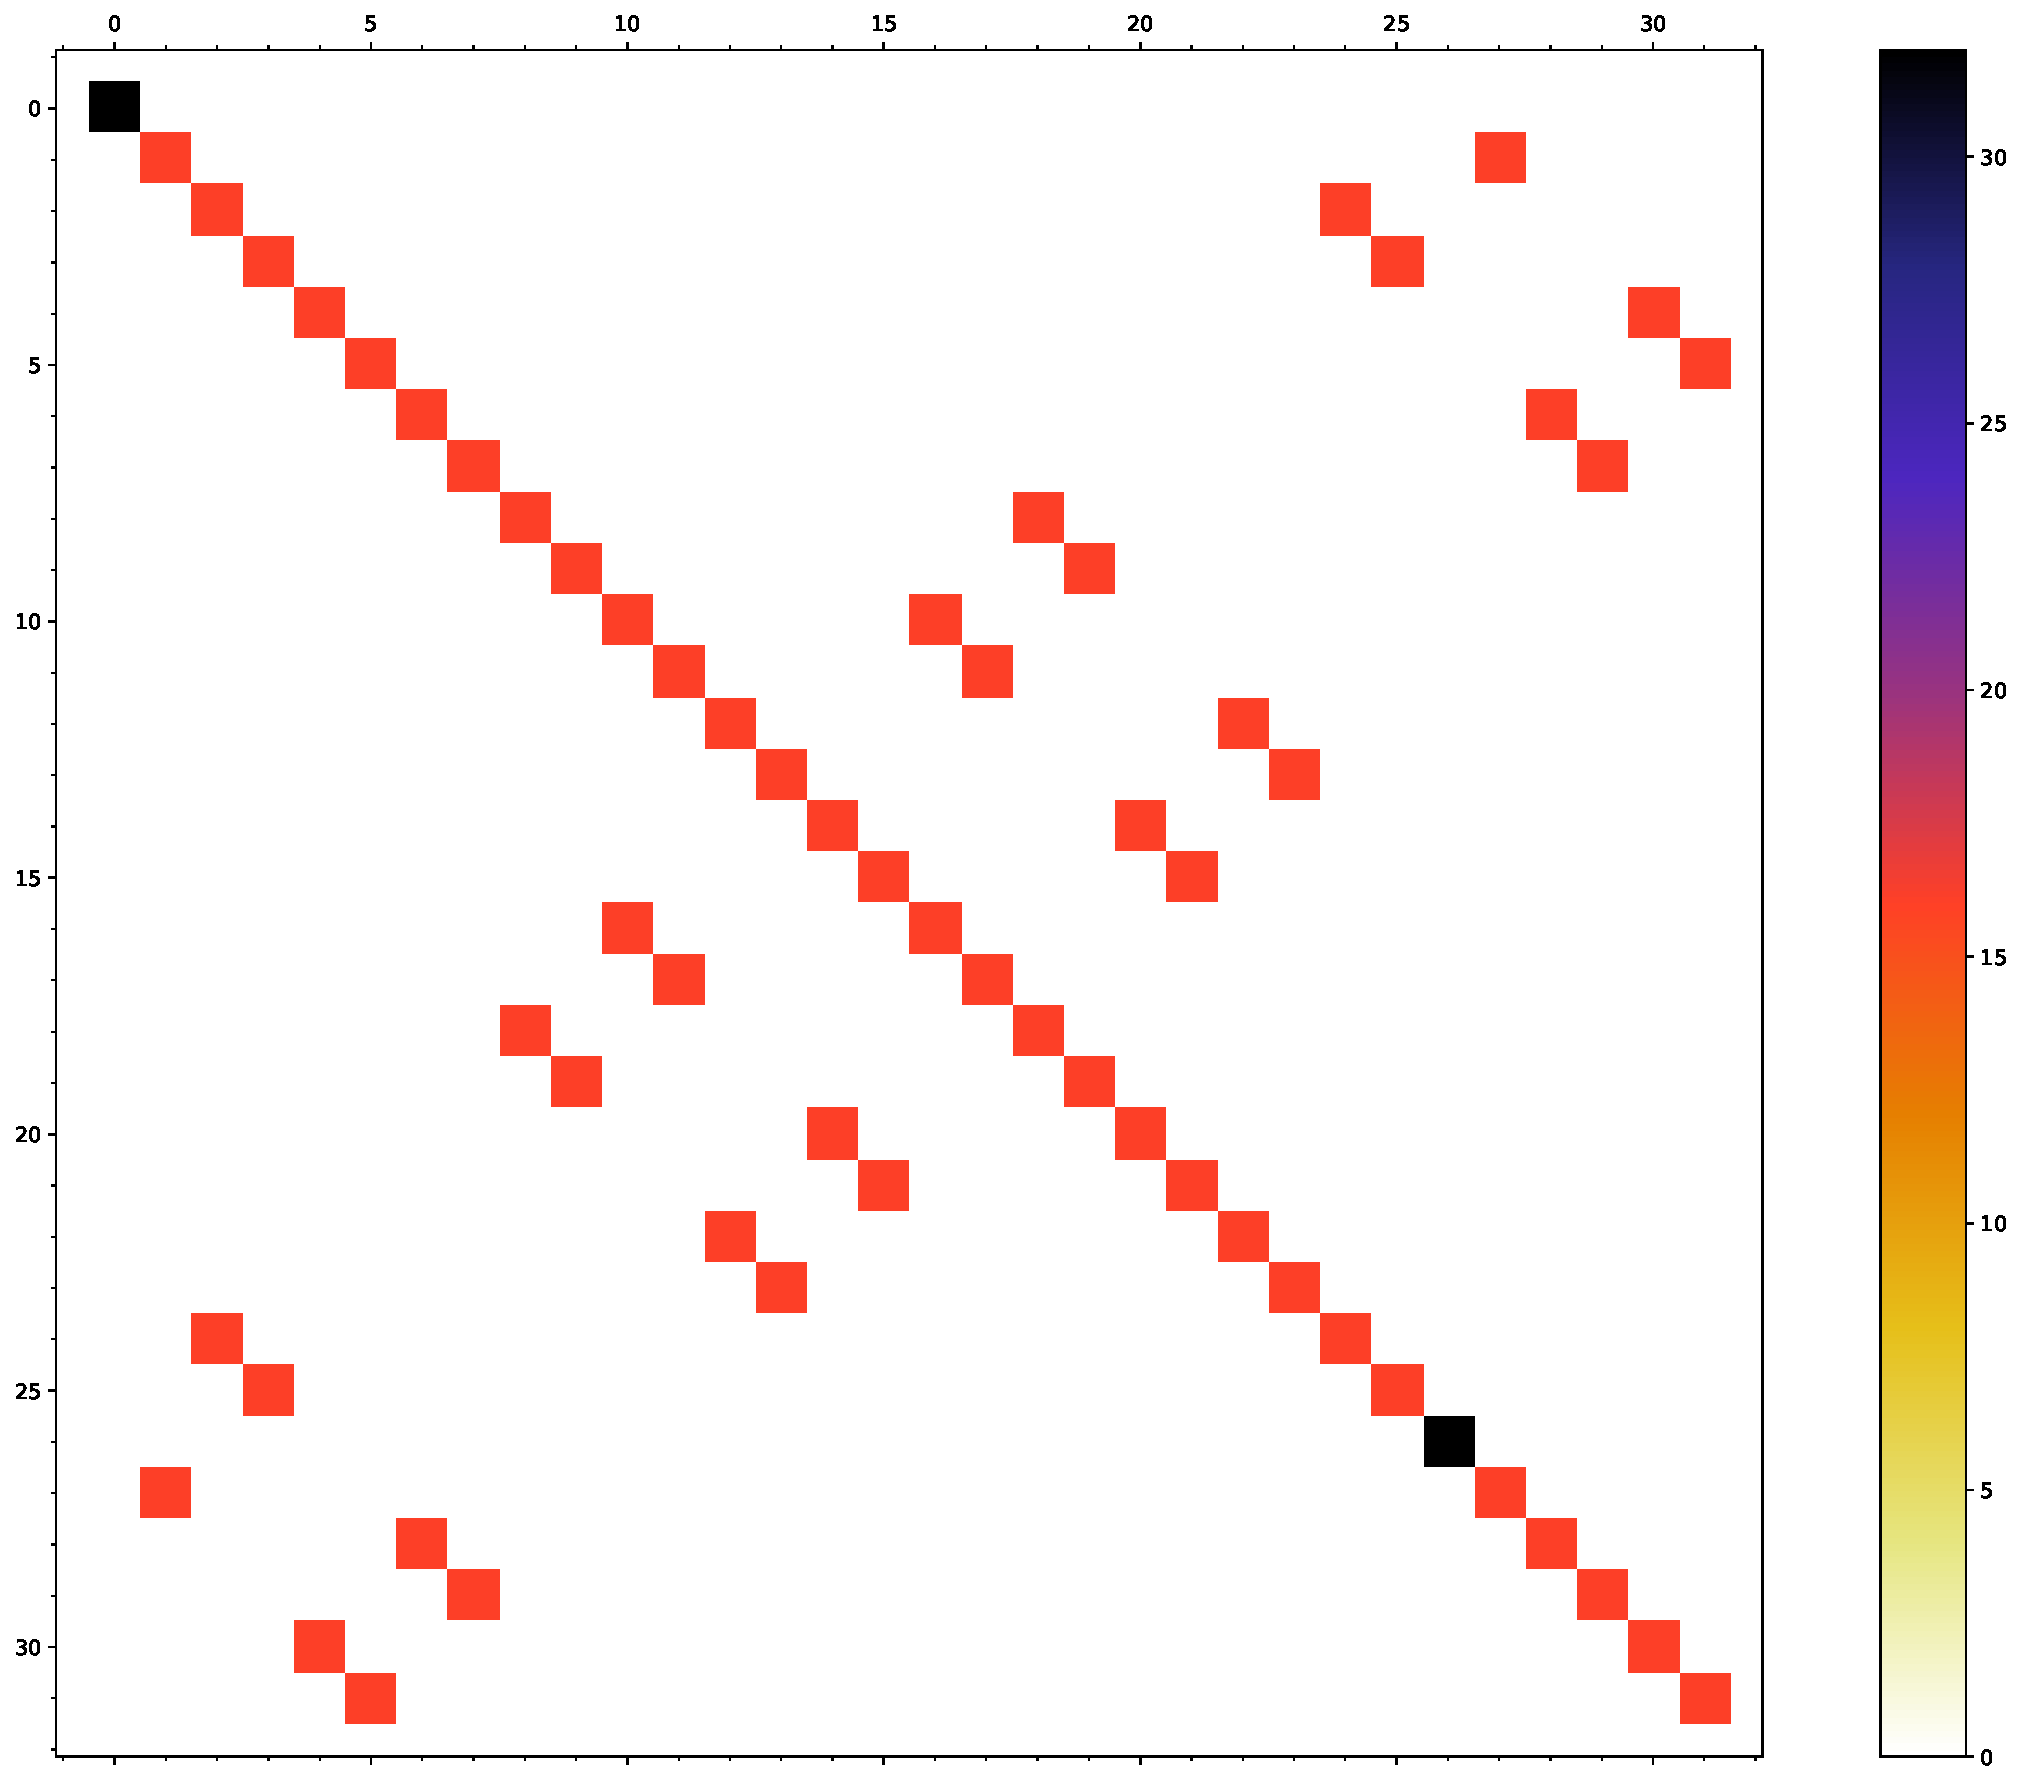
\includegraphics[width=\textwidth]{data/ddt-one-round}
        \end{column}
    \end{columns}
\end{frame}

\begin{frame}{Differential Cryptanalysis}{More rounds}
    \begin{columns}
        \begin{column}{0.49\textwidth}
            \begin{block}{Differences over $r = 3$ rounds}
                \centering
                \begin{forest}
                    for tree={grow=east},
                    [$\alpha$
                        [{$\alpha$}, edge label={node[midway,below,font=\scriptsize] {$\frac{1}{2}$}}, tikz={\node[draw,gray!20,inner sep=0,fit to=tree]{};}
                            [{$\alpha$}
                                [{$\alpha$}]
                                [{$\alpha + k_3$}]
                            ]
                            [{$\alpha + k_2$}
                                [{$\alpha + k_2$}]
                                [{$\alpha + k_2 + k_3$}]
                            ]
                        ]
                        [{$\alpha + k_1$}, edge label={node[midway,above,font=\scriptsize] {$\frac{1}{2}$}}
                            [{$\alpha + k_1$}, edge={thick}, edge label={node[midway,below,xshift=-1mm,font=\scriptsize] {$1$}}, tikz={\node[draw,gray!20,inner sep=0,fit to=tree]{};}
                                [{$\alpha + k_1$}]
                                [{$\alpha + k_1 + k_3$}]
                            ]
                            [{$\alpha + k_1 + k_2$}, edge={dotted}, edge label={node[midway,above,xshift=-1mm,font=\scriptsize] {$0$}}, tikz={\node[draw,gray!20,inner sep=0,fit to=tree]{};}
                                [{$\alpha + k_1 + k_2$}, edge={dotted}]
                                [{$\alpha + k_1 + k_2 + k_3$}, edge={dotted}]
                            ]
                        ]
                    ]
                    %\draw[] (forest cs:l=75mm,s=22.5mm) node[right]{\cref{eqn:impossible_output}};
                    %\draw[] (forest cs:l=75mm,s=7.5mm) node[right]{\cref{eqn:collapsed_output}};
                    %\draw[] (forest cs:l=75mm,s=-12.5mm) node[right]{\cref{eqn:other_output}};
                \end{forest}
            \end{block}
        \end{column}
        \begin{column}{0.49\textwidth}
            \begin{block}{Probabilities of output differences}
                \begin{equation*}
                    \Prob\bracket{\alpha \to \beta} = \begin{cases*}
                        2^{-r}   & if $\beta$ in normal branch\\
                        2^{-r+1} & if $\beta$ in collapsed branch\\
                        0        & if $\beta$ in impossible branch
                    \end{cases*}.
                \end{equation*}
            \end{block}
            \begin{alertblock}{Collapsing}
                How many branches can collapse?
            \end{alertblock}
            \begin{exampleblock}{Once}
                For $r \leqslant n$ rounds and linearly indp.\ round keys this happens only once.
            \end{exampleblock}
        \end{column}
    \end{columns}
\end{frame}

\section{Further Analysis}
\begin{frame}{Further Cryptanalysis}
    \begin{itemize}
        \item Linear Cryptanalysis
        \item Impossible Differentials
        \item Zero Correlation
        \item Invariant Attacks
    \end{itemize}
\end{frame}

\begin{frame}{Conclusion/Questions}{Thank you for your attention!}
    \begin{columns}
        \begin{column}{0.5\textwidth}
            \begin{block}{\bison/}
                \begin{itemize}
                    \item A first instance of the WSN construction
                    \item Good results for differential cryptanalysis
                \end{itemize}
            \end{block}
            \begin{block}{Open Problems}
                \begin{itemize}
                    \item Construction with similar good results for linear cryptanalysis
                    \item Further analysis: division properties
                \end{itemize}
            \end{block}
        \end{column}
        \begin{column}{0.39\textwidth}
        \begin{figure}[!htb]
            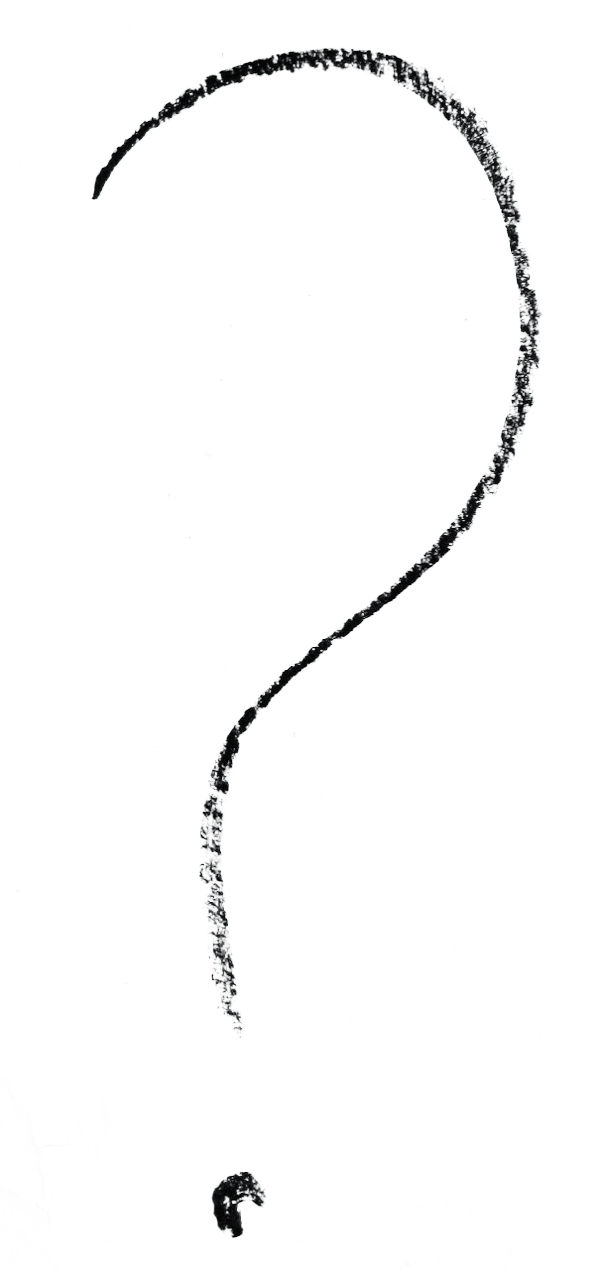
\includegraphics[height=50mm]{data/flickr/questionmark.png}
        \end{figure}
        \end{column}
    \end{columns}
    \blfootnote{\scriptsize Mainboard \& Questionmark Images: flickr}
\end{frame}

\begin{frame}[allowframebreaks]{References}
    \tiny
    \printbibliography{}
\end{frame}
